\documentclass[10pt,a4paper]{article}
\usepackage[utf8]{inputenc} % para poder usar tildes en archivos UTF-8
\usepackage[spanish, es-tabla]{babel} % para que comandos como \today den el resultado en castellano
\usepackage{a4wide} % márgenes un poco más anchos que lo usual
\usepackage[conEntregas]{caratula}
\usepackage{xcolor,colortbl}
\usepackage{todonotes}
\usepackage{graphicx}
\usepackage{subcaption}
\usepackage{algorithm}
\usepackage{algorithmic}
\usepackage{dirtree}
\usepackage{cite}
\usepackage{listings}


\lstset { %
    language=C++,
    backgroundcolor=\color{green!5}, % set backgroundcolor
    basicstyle=\footnotesize,% basic font setting
}

%definations
\definecolor{Gray}{gray}{0.6}
\definecolor{ligthGray}{gray}{0.9}
\newcommand{\mc}[2]{\multicolumn{#1}{|c|}{#2}}

\begin{document}

\titulo{NetworkDEVS}
\subtitulo{Una herramienta de estudio para medelar redes usando DEVS y PowerDEVS}

\fecha{\today}

\materia{Teoría de las telecomunicaciones}

\integrante{Belloli, Laouen Mayal Louan}{134/11}{laouen.belloli@gmail.com}

\maketitle

\tableofcontents
\newpage

\section{Introducción y Motivación}

El presente trabajo se introduce un modelo DEVS de una red funcionando bajo el protocolo TCP/IP encuadrando lo mejor posible cada uno de sus módulos en su correspondiente capa respecto al modelo OSI presentado en la literatura oficial de la materia de teoría de la telecomunicaciones \cite{peterson2007computer}. El trabajo fue desarrollado en el simulador PowerDEVS y pensado como herramienta de aprendizaje para futuros alumnos de la materia.

El principal aporte de este trabajo consiste en la creación de un framework que permite programar y modificar los protocolos de una red de telecomunicaciones para luego simular su comportamiento y obtener feedback instantáneo de los resultados. Además, usando el simulador PowerDEVS, se consigue brindar una interfaz gráfica intuitiva que mapea de forma directa los dispositivos de la red con los módulos del modelo. Esta interfaz gráfica permite también crear distintos escenarios topológicos sin tener que tocar ni una linea de código. 

Por otro lado, esta interfaz gráfica permite modularizar de forma explicita las distintas capas del modelo y su interacción, mapeando los modelos DEVS de cada capa con su capa correspondiente en la red, permitiendo una interacción más tangible y concreta respecto al modelo en capa. De esta forma, se programa cada protocolo en su capa correspondiente, esto no es menor, ya que si bien, teóricamente, los distintos protocolos están separados en capas y las redes pueden ser pensadas en capas, en la realidad, estas capas no existen de forma explicita y hay un salto entre las teorías de redes y los modelos en capas respecto de sus distintas implementaciones prácticas donde las capas terminan mezclándose en varios aspectos. Este modelo, permite a los alumnos hacer trabajos prácticos donde implementar los protocolos manteniendo explicitas las capas y por ende, acercando la teoría y la práctica de las redes de telecomunicaciones.

Si bien, el modelo realizado es un modelo DEVS (Discrete EVent System Specification), el mismo fue pensado para que no sea necesario más que una breve introducción a DEVS, por lo que mismo personas sin ninguna experiencia en DEVS deberían ser capases de poder utilizar el simulador, el modelo y el framework general propuesto en este trabajo.

\section{Objetivos}

Los objetivos de este trabajo se pueden dividir en varias partes:
\subsection{Desarrollar un framework para modelos de redes}

Como ya fue mencionado en la introducción, uno de los principales objetivos de este trabajo es desarrollar un framework, que permita fácilmente implementar protocolos de red, validarlos y experimentar con ellos mediante Simulación de Eventos Discretos (DES). Ests herramienta permite testear los protocolos implementados de forma sencilla y rápida. Obteniendo una herramienta útil, tanto para el estudio de las redes de telecomunicaciones como para la investigación en el área. 

La creación de un modelo que sirva como framework, tiene por objetivo factorizar y estandarizar las partes comunes a todos los protocolos, estás partes comunes provienen de las propiedades inherentes a los dispositivos físicos en los cuales los protocolos están corriendo, y de los estándares actualmente utilizados que permiten obtener robustez y compatibilidad entre distintas implementaciones que puedan existir en distintas partes de una red. Estas abstracciones encapsuladas en el modelo framework presentado, permiten al modelador, concentrarse plenamente en su protocolo y permite la reutilización y compatibilidad de distintos modelos que pueden luego ser combinados en un único modelo de una red que funcione bajo distintos protocolos, permitiendo así el estudio de la compatibilidad, homogeneidad y efectividad de los protocolos implementados.

\subsection{Modelar una red UDP/IP básica}

Por otro lado, este trabajo pretende implementar un modelo básico de una red UDP/IP que permita cubrir los protocolos mínimos e indispensables para permitir enviar mensajes entre distintos dispositivos. Este modelo no tiene como intensión implementar todas las partes, ni cubrir todos los protocolos de forma completa, por lo que temáticas como la fragmentación de paquetes, congestión de tráfico, manejo de errores, Dinamic Host Configuration Protocol (DHCP) \cite[p.~231]{peterson2007computer}, Routing Information Protocol (RIP)\cite[p.~243]{peterson2007computer} y Spanning tree protocol \cite[p.~194]{peterson2007computer} quedan fuera del alcance de este trabajo, siendo los mismos posibles trabajos futuros.

También se implementó un modelo de switch que utiliza el protocolo de Datagramas \cite{petersonSwitchDatagram} utilizando una forwarding table para enviar los Frames por la interface correspondiente. 

\subsection{Mapeo entre el modelo UDP/IP y el modelo OSI}

En este trabajo, también pretendemos mostrar como se pueden implementar los distintos protocolos del modelo UDP/IP encuadrandolos en un modelo en capas OSI. Para esto, varias decisiones tuvieron que tomarse, siendo tal vez la más difícil, decidir en que capa implementar el protocolo ARP \cite[p.~228]{peterson2007computer}. Para tomar estas decisiones, se tomaron siempre como referencia los textos del libro oficial de la materia \cite{peterson2007computer}. Se intentó también separar lo mejor posible las tareas de cada capa de forma tal que cada una de ellas pueda ignorar lo más posible la existencia de la/las capa/s inferior/es.

\section{Introdución a DEVS}
\section{Introducción a PowerDEVS}
\section{Arquitectura}

\subsubsection{Arquitectura general}
La arquitectura general del modelo propuesto en este trabajo tiene por principal objetivo ofreser un framework donde se pueda facilmente desarrollar protocolos, para esto, se concentra en resolver varios puntos principales:

\begin{itemize}
\item Estandarizar la comunicación entre las capas de forma de conseguir consenso entre los distintos modeladores que usen esta herramienta, y que facilite una comprensión herarquica y organizada del modelo entero para los lectores nuevos.
\item Implementar todas aquellas partes generales a todos los modelos de protocolos de forma que solo sea necesario consentrarse en el protocolo a implementar.
\item intentar minimizar lo más posible la necesidad de tener conocimientos avanzados sobre DEVS a la hora de utilizar la herramienta.
\end{itemize}

La arquitectura consiste en un modelo acoplado "dispositivo" de $N$ capas, con $N > 0$ de forma que cada capa $i, i \in [1,..,N]$ se comunica con las capas $i+1$ e $i-1$ utilizando $8$ canales de comunicación distintos:

\begin{itemize}
\item Output port 0: Envio de datos a la capa $i+1$.
\item Output port 1: Envio de controles a la capa $i+1$.
\item Output port 2: Envio de datos a la capa $i-1$.
\item Output port 3: Envio de controles a la capa $i-1$.
\item Input port 0: Recepción de datos de la capa $i+1$.
\item Input port 1: Recepción de controles de la capa $i+1$.
\item Input port 2: Recepción de datos de la capa $i-1$.
\item Input port 3: Recepción de controles de la capa $i-1$.
\end{itemize}

Dado que no siempre sucede que en un dispositivo de la red, exista un solo modulo por capa, y dado que los puertos de salida y entradas estan pensados para comunicarse con un solo modelo en la capa superior/inferior. Es necesario usar modelos demultiplexers que permitan redirigir los mensajes salientes por un puerto al modelo correspondiente de entre todas las posibles opciones. También, es necesario usar modelos multiplexers para que los múltiples modelos de la capa superior o inferior puedan enviarle mensajes al modulo. Ejemplos de estos son: un host que tenga varias aplicaciones enviando datos a travez de distintos sockets y en ese escenario habria más de un módulo en la capa de aplicación (capa siete del modelo OSI) de ese host, un router  que tenga más de una interfaz (una por cada sub-red a la cual esté conectado), contando con más de un modulo en la capa de linkeo (capa dos del modelo OSI). \\

Las capas $1$ y $N$ usan la misma arquitectura que el resto de las capas y tienen definidos los mismos puertos. Como que existe solo un medio de comunicación entre dispositivos y tanto datos como controles se envian por ese medio, entonces el modelo acoplado "dispositivo" tiene solo un puerto de salida y un puerto de entrada destinado a enviar datos de cualquier tipo, y queda en el modelador decidir que puerto o puertos de salida de la capa $1$ conectar con el puerto de salida del modelo acoplado y que puerto o puertos de entrada de la capa $1$ comunicar con los el puerto de entrada para datos. Por otro lado, el input requerido por la capa $N$ (comunmente el input que indica los pedidos del usuario de enviar o recibir datos) se puede conectar con modelos generadores que pueden estar situados tanto adentro como afuera del modelo acoplado. Lo mismo ocurre con el output generado por la capa $N$ para las capas superiores que no existen; este output puede ser recibido por modelos que lo guardan en archivos y estos modelos también pueden estar situados tanto adentro como afuera del modelo acoplado \\

Distintos dispositivos de la red pueden tener distintas cantidades de capas, por lo cual, la cantidad de capas existente puede variar entre los distintos modelos de cada dispositivo dentro de una misma red. Los hosts por ejemplo, suelen tener hasta la capa siete, mientras que los routers comunes llegan a la capa tres y los switches a la capa dos. \\

La Figura \ref{figure:general architecture} muestra la arquitectura general recien explicada en un modelo de una red con un host y un router, en el mismo se pueden ver: los multiplexers y demultiplexers, modelos con distintas cantidades de capas y las conexiones entre capas utilizando los distintos puertos. \\

\begin{figure}[htbp]
    \centering
    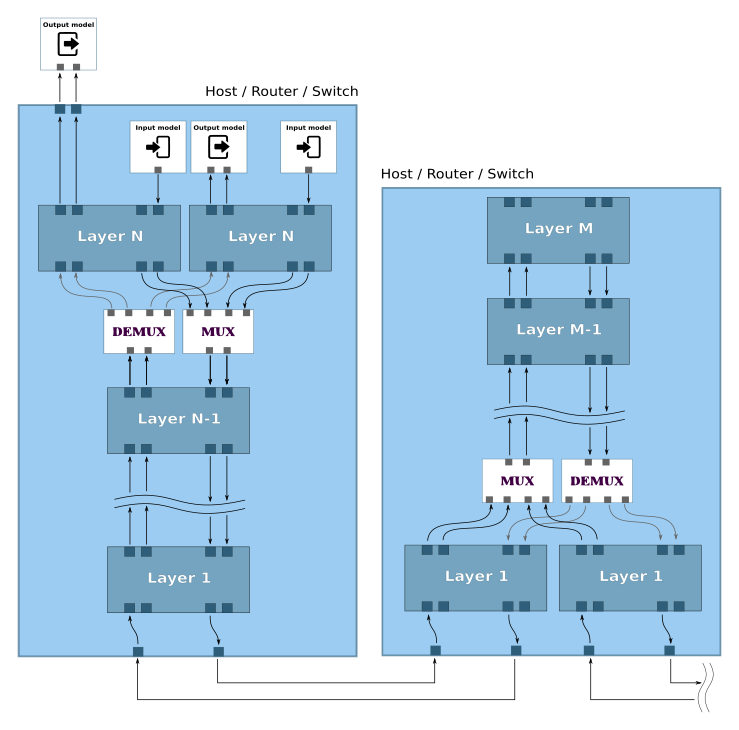
\includegraphics[width = 0.5\textwidth]{img/png/general_architecture.png}
    \caption{Arquitectura de un modelo en NetworkDEVS con dos dispositivos (un host y un reouter de N y M capas correspondientemente).}
    \label{figure:general architecture}
\end{figure}

\newpage

\subsubsection{Arquitectura de las capas}

La arquitectura de las capas está implementado en un modelo template llamado Layer del cual se puede realizar herencia para heredar su estructura. Esta estructura permite abstraer al protocolo de todo el modelo correspondiente al dispositivo, en otras palabras, esta estructura ya modela las propiedades de un dispositivo generico, esto implica manejar el envio y recepción de mensajes a y de otras capas. Para manejar la entrada y salida de mensajes se utilizan colas FIFO; Cada vez que hay un mensajes entrante, el mismo es encolado en la cola de entrada correspondiente y el protocolo los va desencolando y atendiendo de uno o de a muchos dependiendo su implementación, la estructura ya está armada de forma que mientras no halla mensajes por procesar mantiene al modelo pasivado (en estado IDLE) y mientras que hay mensajes por procesar lopea para ir atendiendolos a todos hasta que no halla más mensajes a procesar, momento en el que el modelo se vuelve a pasivar. Por otro lado, cada vez que se quiere enviar un mensaje, el mismo solo debe ser encolado en la cola de mensajes salientes correspondiente dependiendo de si es un mensaje de datos o control a la capa superior o inferior, luego el simulador cuando el protocolo termina el procesamiento actual se encarga de loopear entre las colas de salida para enviar todos los mensajes que hallan sido encolados. La Figura \ref{figure:layer general architecture} muestra la arquitectura deneral de una capa cualquiera y la Figura \ref{figure:processing flow} muestra el flujo de procesamiento generado por el modelo template cuando es extendido agregandole un protocolo.

\begin{figure}[htbp]
    \centering
    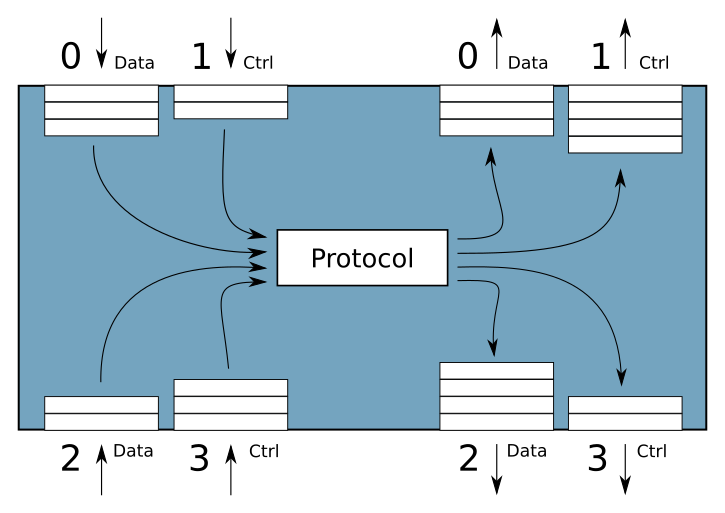
\includegraphics[width = 0.4\textwidth]{img/png/layer_architecture.png}
    \caption{Arquitectura de una capa en NetworkDEVS.}
    \label{figure:layer general architecture}
\end{figure}

\begin{figure}[htbp]
    \centering
    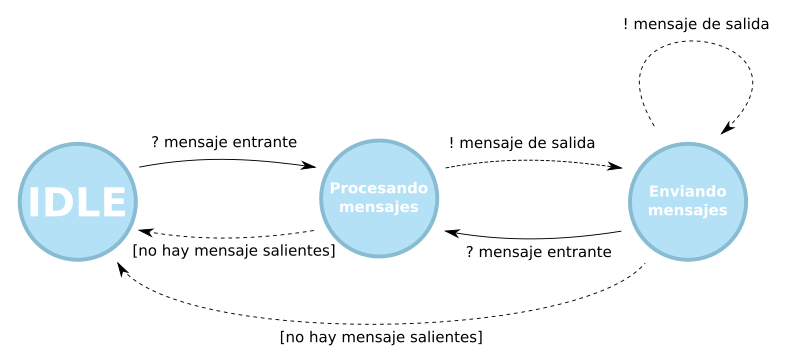
\includegraphics[width = 0.6\textwidth]{img/png/processing_flow.png}
    \caption{Flujo de procesamiento de una capa que extiende al modelo template Layer.}
    \label{figure:processing flow}
\end{figure}

\section{Como usar el template}

Todo el modelo está implementado en C++ y la forma de usar el template es mediante la implementación de herencias. Para poder comprender como utilizarlo, primero introduciremos la estructura de archivos del framework. \\

\dirtree{%
.1 NetworkDEVS.
.2 libs.
.3 logger.h.
.3 message\_queue.h.
.3 parser.h.
.2 structures.
.3 bastract\_types.h.
.3 app.h.
.3 ip.h.
.3 ipv4.h
.3 link.h.
.3 mac.h.
.3 socket.h.
.3 sw.h.
.3 swp.h.
.3 udp.h.
.2 templates. 
.3 layer.h.
.3 demultiplexer.h.
.3 multiplexer.h.
.2 top.pdm.
.2 top.pds.
.2 top.stm.
}

\medskip

La carpeta \textit{structures} es la que contiene las definiciones de todos los tipos de datos que vienen por defecto con el framework, algunos de ellos fueron implementados exclusivamente para el modelo presentado en este trabajo, pero todos pueden ser utilizados y están incluidos por el modelo template Layer que introduciremos a continuación. Los tipos de datos están implementados usando structs y casi todos heredan de dos tipos abstractos definidos en \textit{abstract\_types.h} que sirven como organizadores, de esta forma quedan están separados entre los que son Data y los que son Headers. Cada tipo de dato definido cuenta con documentación en el código en formato Doxigen y la misma fue exportada y se encuentra disponible en el apendice de este documento. \\

Todos los tipos de datos estan implementados en namespaces que sirven como organizadores, para cada capa existente debe existir un namespace y los tipos de datos inherentes a esa capa (por más que otras capas lo usen) tienen que estar definidos dentro del namespace. Si se implementan nuevas capas, se deben crear sus correcpondientes namespaces a menos que no halla tipos de datos correspondientes a la capa. De está forma se evitan las ambiguedades, que son muy recurrentes en el ambito de las redes.

\subsection{Como heredar el modelo layer}

El modelo Layer es el modelo template que contiene toda la implementación correspondiente a la arquitectura general de una capa. El mismo es un modelo que cuenta con 4 tipos de datos templates a instanciar y 4 tipos de datos template con instanciación por defecto si no se explicitaran otros tipos para ellos. Estos tipos a instanciar son los tipos de los mensajes que envian y reciben los puertos y los tipos con los cuales se definen las colas. Por defecto se asume que los puertos de entrada y salida del mismo tipo de mensajes (Datos o Control) para y desde la misma capa, tienen el mismo tipo. Es por esto que hay solo 4 tipos template que deben ser instanciados obligatoriamente, mientras que los restantes cuatro se mapean por defecto con los primeros 4 para conseguir sus tipos.\\

El modelo Layer tiene la siguiente forma:
\begin{lstlisting}
template <typename DH, typename CH, typename DL, typename CL, 
	typename DH2 = DH, typename CH2 = CH, typename DL2 = DL, typename CL2 = CL>
class Layer: public Simulator { 

protected:
  // Logger
  Logger logger;

  // Input queues
  std::queue<DH> higher_layer_data_in; // Input Port 0
  std::queue<DL> lower_layer_data_in;  // Input Port 1
  std::queue<CH> higher_layer_ctrl_in; // Input Port 2 
  std::queue<CL> lower_layer_ctrl_in;  // Input Port 3
  
  // Output queues
  msg::queue<DH2> higher_layer_data_out; // Output Port 0 
  msg::queue<DL2> lower_layer_data_out;  // Output Port 1
  msg::queue<CH2> higher_layer_ctrl_out; // Output Port 2
  msg::queue<CL2> lower_layer_ctrl_out;  // Output Port 3

  Event output;

  double next_internal;
  double last_transition;
  double infinity = std::numeric_limits<double>::max();
  bool queuedMsgs() const { ... }

public:

  Layer(const char *n): Simulator(n) {};
  void dint(double t) { .... }
  void dext(Event x, double t) { .... }
  
  virtual void dinternal(double t) {}
  virtual void dexternal(double t) {}
};
\end{lstlisting}

El template cuenta con dos métodos virtuales que están definidos e implementados como funciones que no hacen nada, estos métodos son los que deben ser sobre escritos para implementar el protocolo. Siempre que haya mensajes por procesar en las colas de entradas, el modelo llama al método \textit{internal} en la cual se deben procesar dichos mensajes, al finalizar dicha función, el modelo Layer mira las colas de salidas para ver si hay mensajes a enviar y los envia, si al finalizar este proceso sigue habiendo mensajes por procesar en la cola de entrada, se volverá a llamar a esta función respetando el formalismo DEVS de forma de seguir procesando mensajes, este proceso se repite indefinidamente hasta que no haya mas mensajes por procesar y cuando esto ocurre, el modelo se pasiva a la espera de nuevos eventos externos. \\

El método virtual \textit{dexternal} existe por si se desea implementar codigo que se ejecute cada vez que ocurre un evento externo para modificar el estado de las variables internas del protocolo o por algún otro propósito. Esto no es recomendado para desarrolladores no familiarizados con el formalismo DEVS ni con PowerDEVS. \\

\textbf{Nota:} Como se puede observar existen las funciones \textit{dint} y \textit{dext} que son las funciones exigidas por el simulador para ejecutar correctamente las transiciones interna y externa correspondientes al formalismo DEVS, el modelo Layer ejecuta en esas funciones todo el código relativo a la arquitectura presentada y llama a los métodos virtuales \textit{internal} y \textit{dexternal} que es sobre escrito por el modelador para ejecutar el protocolo implementado. De esta forma se consigue abstraer lo más posible al modelador del formalismo DEVS convirtiendo esta herramienta en una herramienta viable para el uso de estudio, mismo con alumnos no familiarizados en DEVS ni DES. 

\subsection{Como enviar y recibir mensajes entre las capas}

Todos los mensajes que llegan al modelo de una capa son recibidas por uno de los cuatro siguientes puertos dependiendo de donde provenga el mensaje:
\begin{itemize}
\item std::queue$<DH>$ higher\_layer\_data\_in:  Input Port 0
\item std::queue$<DL>$ lower\_layer\_data\_in:   Input Port 1
\item std::queue$<CH>$ higher\_layer\_ctrl\_in:  Input Port 2 
\item std::queue$<CL>$ lower\_layer\_ctrl\_in:   Input Port 3
\end{itemize}

Como ya fue mencionado y como se puede observar en la definición de las colas, los tipos template instanciados son los tipos de los mensajes recibidos desde las capas superior e inferior. Es importante que los mensajes recibidos sean efectivamente de este tipo, porque el simulador PowerDEVS envia mensajes como \textbf{void *} y los mismos son casteados a su tipo correspondientes una vez recibidos por el modelo receptor, por lo que si los tipos no corresponden se generará un excepción en tiempo de ejecución. \\

Para procesar los mensajes, dentro del método \textit{internal}, los mismos deben ser desencolados, es importante que se desencolen, ya que en caso contrario el mismo seguirá estando en la cola y el modelo volverá a producir una transición interna y llamar de nuevo al método \textit{internal} procesando dos o más veces el mismo mensaje. Reprocesar un mensaje multiple veces probablemente esté mal, pero tal vez es lo deseado por el protocolo, pero hay que tener en cuenta que una de las pocas exigencias del formalizmo DEVS es que no ocurran infinitos eventos en un mismo momento del tiempo virtual, y como el modelo sigué generando transiciones internas mientras haya mensajes por procesar, si los mensajes no son nunca desencolados, se generarán infinitas transiciones internas y eso produce un modelo DEVS ilegítimo que cuelgué al simulador. \\

Para enviar mensajes las colas utilizar son las siguientes:
\begin{itemize}
\item msg::queue$<DH2>$ higher\_layer\_data\_out: Output Port 0 
\item msg::queue$<DL2>$ lower\_layer\_data\_out:  Output Port 1
\item msg::queue$<CH2>$ higher\_layer\_ctrl\_out: Output Port 2
\item msg::queue$<CL2>$ lower\_layer\_ctrl\_out:  Output Port 3
\end{itemize}

Como se puede observar, los nombres de los tipos a instanciar son iguales a los de las colas de entrada, esto es porque los mismos por defecto se instancian usando los mismos tipos a menos que en la declaración de la herencia se especifique lo contrario, esto es así ya y se considera buena práctica que el tipo de datos que intercambian dos capas por un canal de comunicación sea siempre el mismo en ambas direcciónes, facilitando la reutilización y comprensión de los modelos por parte de otras personas. \\

Para encolar un mensaje en la cola de de salida correspondiente se debe utilizar el metodo \textit{push(MSG mensaje)}. De la misma forma que el modelo Layer se encarga de encolar los mensajes en la cola de entrada correspondiente dependiendo el puerto por donde llegó el mensaje, el mismo se encarga de enviar los mensajes encolados en las colas de salidas por el puerto correspondiente a cada cola y desencolar el mismo. \\

El tipo de datos msg::multiplexed<typename MSG> sirve para enviar mensajes que van a ser demultiplexados por un modelo demultiplexer<typename MSG>. El mismo cuenta con los campos \textit{message} e \textit{interface} que son utilizados para asignar el mensaje y el identificador del destinatario. Luego solo resta utilizar un modelo demultiplexer, setear correctamente sus parametros en la IDE de PowerDEVS, y conectar correctamente sus puertos de entrada y salida con el modelo de origen y los modelos de destino. La Figura \ref{figure: demultiplexer} muestra como es el mapeo de los puertos del demultiplexer. \\

\todo[inline]{PONER FIGURA DEL DEMULTIPLEXER}

El campo \textit{interface} le indica al demultiplexer por que puerto enviar el mensaje, por lo que es importante conectar correctamente los puertos de salida del demultiplexer correctamente con todos los destinatarios. Para no tener que usar un demultiplexer para los mensajes de datos y otro demultiplexer para los mensajes de controles, el modelo demultiplexer cuenta con dos puertos de entrada (datos y controles) y envia los mensajes por los puertos pares si son datos y por puertos impares si son controles. De esta forma un mensaje de control que llega con interface $i$ es enviado por el puerto $2*i+1$ y un mensaje de datos que llega con interface $i$ es enviado por el puerto $2*i$.

\subsection{Como implementar el protocolo de una capa (internal/external functions)}
\section{Como agregar una capa}
\section{Como modificar un protocolo}
\section{Input/output del modelo}
\section{Logger}
\section{Case study: escenario implementado}
\section{Protocolos implementados}
\subsection{UDP}
\subsection{IP}
\subsection{ARP}
\subsection{SWP}
\subsection{Datagram protocol}
\section{Resultados}
\section{Conclusiones}
\section{Trabajo futuro}
\section{References}
\bibliographystyle{plain}
\bibliography{references}

\end{document}